\chapter{Introduction}
\label{chp:introduction} 

\section{About the Thesis}

\subsection{Long Term Goal and Previous Work}

\subsubsection{The Topic - Mobile Autonomous Robot}

The robot system that was used in this project has been developed over the course of many preceding master and specialization projects. The long term goal of these projects is to develop mobile autonomous robot concepts for maintenance and inspection on topside offshore installations. The topic is given by Professor Tor Onshus at \ac{ITK}. A description of this topic\footnote{\url{http://folk.ntnu.no/onshus/Oppgaver.htm}}, suggests some possible applications for such a robot: 

\begin{itemize}
	\item The robot could serve in a supporting role as a part of \ac{IO}.
	\item It can also be used to prepare an unmanned topside offshore installation before the arrival of a maintenance crew, by performing safety checks and preparing the helicopter landing pad.  
	\item Allow personnel to perform remote inspection and maintenance through telepresence.
	\item  In combination with \ac{VR}, the robot could be used for training purposes. 
\end{itemize}

\subsubsection{Telepresence and the Robotic Arm}

The system in its current form is built around a robot manipulator arm, SCORBOT-ER4u. Kristian Saxrud Bekken focused on improving previous work on the system, which was done as early as 2005\cite{bekken}. Bekken's work comprise telepresence through a stereo video transmission, a collision avoidance system for the robot arm and an improved \ac{HMI} implementation.

\subsubsection{Building the Mobile Platform}
During the spring of 2013, Petter Aspunvik devoted his master's project to develop a mobile base for the robotic arm\cite{aspunvik}. Aspunvik's thesis has served as a user manual for many of the robot systems in the early stages of this project. The current motor control firmware is based on Aspunvik's implementation.

\subsubsection{Simultaneous Localization and Mapping}

In parallel to Aspunvik's project, Mikael Berg developed a solution for \ac{SLAM} and autonomous navigation for the same robot\cite{berg}. His software is programmed in Google's Go language, and runs on Windows 7 within the pre-installed on-board computer. The resulting system successfully utilized Hector SLAM with a LIDAR and odometry from two encoder wheels for 2d navigation and \ac{SLAM}. Berg considered to create a solution based on \ac{ROS} which requires a Linux platform. In the end, he opted to target the Windows platform as this is the only operating system which is compatible with the robotic arm. The ''future work''-section in Berg's thesis suggests improvements in the form of 3d obstruction detection, because the LIDAR is limited to detection in a plane. He also mentions object recognition and dynamic re-planning as possible extensions. 

\subsubsection{Last Year's Specialization Project}

This authors specialization project\cite{lindrup} presented an obstruction detector based on two unsynchronized IP-cameras and a stereo matching algorithm in \ac{OpenCV}. Because the cameras were unsynchronized, the system would become useless whenever there is relative motion between the robot and the surroundings. The obstruction detector lacked a critical feature: a floor filter to separate the ground from potential obstructions. The implementation presented in this master's project is unrelated to the preceding specialization project, except for some useful functions in c++.

\section{Implementation Overview}

\begin{figure}[p]
	\centering
	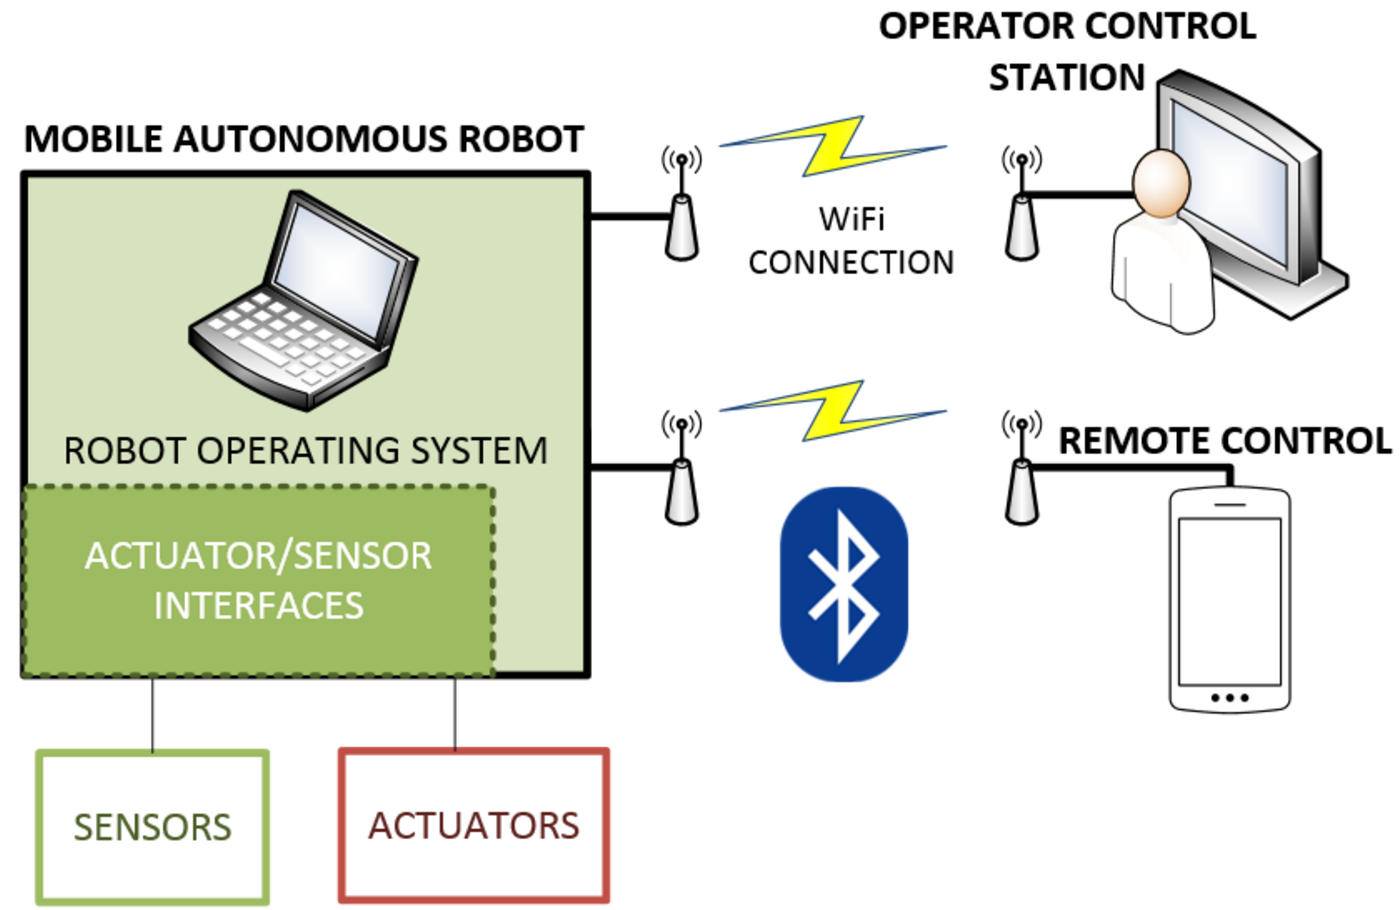
\includegraphics[width=0.8\textwidth]{conseptDrawing}
	\caption{System Concept. An on-board computer using \ac{ROS} to handle actuators and sensors. Remote operation is available through an \ac{OCS} or a hand-held device with Bluetooth.}
	\label{fig:conseptDrawing}
\end{figure}

\section{Thesis Structure}